\label{peripherals}
%%%%%%%%%%%%%%%%%%%%%%%%%%%%%%%%%%%%%%%%%%%%%%%%%%%%%%%%%%%%%%%%%%
%%%%%%%%%%%%%%%%%%%%%%%%%%%%%%%%%%%%%%%%%%%%%%%%%%%%%%%%%%%%%%%%%%

\subsection{Ports}
Un processeur \acrshort{IA-32} a la possibilité de transférer des données en utilisant
les ports d'entrée/sortie. Ces ports sont utilisés par le processeurs pour communiquer
avec des périphériques. Il peuvent être utilisés pour envoyer et recevoir des données
(par exemple un \textit{timer} va utiliser les ports d'entrée/sortie pour envoyer
son état). Les ports peuvent aussi être utilisés pour contrôler un péripéhrique
à partir de registres de contrôle (par exemple avec un controlleur de disque) \cite{ref64}.
Etant donné que nous ne sommes pas sur du vrai \textit{hardware}, QEMU va se charger
d'émuler les différents périphériques utilisés par un processeur Intel 32-bits. \\

Les ports d'entrées/sorties sur architecture x86 se situent dans un espace d'adresses
séparé de la mémoire physique. Cet espace permet d'adresser 64000 (soit $2^{16}$)
ports de 8 bits. Les ports sont donc adressés sur 16 bits mais  il n'est pas possible
d'écrire dans un \acrshort{pio} de la même manière que l'on écrirait dans la mémoire
(avec une instruction  \mintinline{text}{MOV}) car nous sommes dans deux
espaces d'adresses différents. Ainsi, le \acrshort{cpu} utilise des instructions speciales
pour accéder aux \acrshort{pio}. Ces instructions sont les instructions
\mintinline{text}{IN} et \mintinline{text}{OUT}. \mintinline{text}{IN} permet de lire
tandis que \mintinline{text}{OUT} permet d'écrire. A noter que l'adresse du port
doit toujours être spécifiée dans le registre \mintinline{text}{dx} et la lecture
et l'écriture se font toujours avec les registres \mintinline{text}{ax/al} \cite{ref42}. \\

\begin{multicols}{2}
    [
    Exemple de lecture et d'écriture dans un port d'entrée/sortie :
    ]
    Ecrire 4 dans le port 0x2A :
    \begin{minted}[fontsize=\footnotesize,tabsize=4]{text}
    mov dx, 0x2A
    mov al, 4
    out dx, al
    \end{minted}
    \columnbreak
    Lire un octet depuis le port 0x2A :
    \begin{minted}[fontsize=\footnotesize,tabsize=4]{text}
    mov dx, 0x2A
    in  byte al, dx
    \end{minted}
\end{multicols}

Il existe une autre méthode pour écrire dans les ports utilisant le même bus d'adresse
pour la mémoire physique et pour les périphériques. Cette méthode consiste à
\textit{mapper} les ports d'entrées/sorties dans la mémoire physique (\acrshort{mmio}).
En écrivant dans la zone reservée aux ports, on écrirait alors directement dans
les ports et pas dans la mémoire physique. Le \textit{kernel} développé utilise
la première méthode (\acrshort{pio}).

%%%%%%%%%%%%%%%%%%%%%%%%%%%%%%%%%%%%%%%%%%%%%%%%%%%%%%%%%%%%%%%%%%
%%%%%%%%%%%%%%%%%%%%%%%%%%%%%%%%%%%%%%%%%%%%%%%%%%%%%%%%%%%%%%%%%%

\subsection{Interruptions et Exceptions}
\subsubsection{Principe général}
Les interruptions et les exceptions sont des évenements qui indiquent que l'attention
du processeur est demandée quelque part soit dans le code, soit par un périphérique.
Il existe deux types d'interruptions, les interruptions logicielles et les interruptions
matérielles. Les exceptions sont générées par le processeur mais diffèrent des
interruptions logicielles. Une interruption peut arriver à n'importe quel moment
en réponse au signal d'un périphérique ou bien si le processeur le demande
avec l'instruction \mintinline{text}{INT} (interruption logicielle). Une exception
est levée lorsque le processeur détecte une erreur à l'exécution d'une instruction
(par exemple une division par 0). Quand une interruption ou une exception
a lieu, une routine logicielle est appelée (\acrshort{isr}). Les processeurs \acrshort{IA-32}
supportent jusqu'à 256 interruptions dont les 32 premières sont reservées aux exceptions
(voir figure \ref{table_int_exc}) \cite{ref42,ref66}. \\

\begin{figure}[!h]
  \centering
  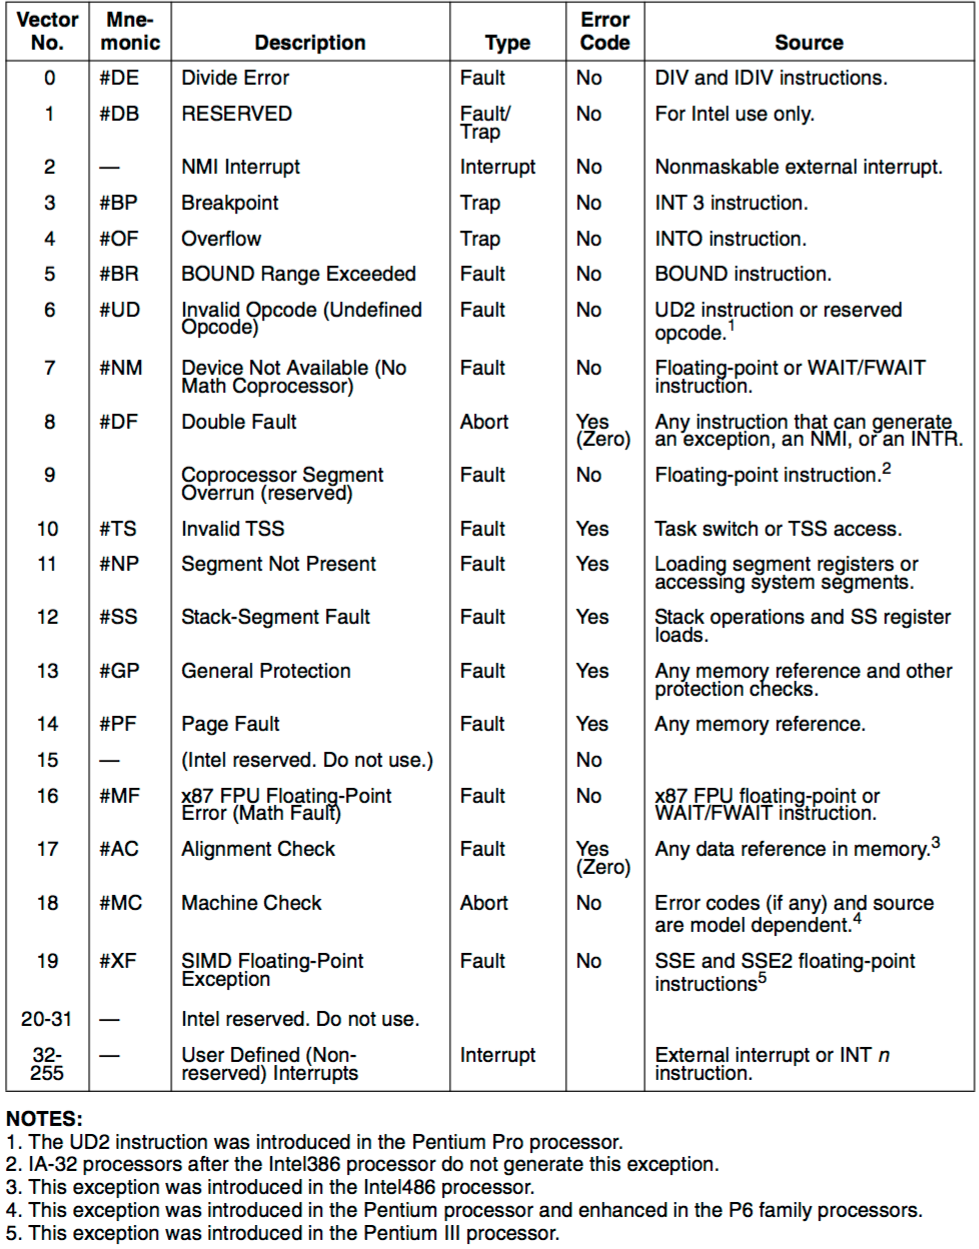
\includegraphics[scale=0.39]{images/table_int_exc.png}
  \caption{Table des interruptions et exceptions sur \acrshort{IA-32}}
  \label{table_int_exc}
\end{figure}

Comme vu précedemment, une interruption logicielle peut être exécutée par le
processeur avec l'instruction \mintinline{text}{INT}. L'instruction \mintinline{text}{INT}
suivie du numéro d'interruption sur 8 bits déclenchera l'interruption en question.
Par exemple, l'instruction \mintinline{text}{INT 0x30} déclenchera l'interruption
48. Au moment de l'appel à l'instruction \mintinline{text}{INT}, le pointeur
d'instruction va sauter à l'adresse du code contennant la routine d'interruption
correspondant au numéro d'interruption logicielle specifiée. C'est la table des
descripteurs d'interruption (\acrshort{idt}) qui permet de définir l'adresse du
code à exécuter pour chaque numéro d'interruption (que ce soit une interruption
logicielle, matérielle ou une exception). A noter aussi que les interruptions
logicielles sont synchrone étant donné qu'elles sont exécutées par le processeur,
contrairement aux interruptions matérielles qui sont asynchrones (exécutées par
les périphériques, elle peuvent arriver à n'importe quel moment). \\

Nous avons vu que les interruptions matérielles étaient générées par le \textit{hardware}.
Il existe deux types d'interruptions matérielles, les \acrshort{nmi} (\textit{Non Maskable
Interrupt}) et les \acrshort{irq} (Interrupt Request). Une \acrshort{nmi} indique
qu'un problème est survenu au niveau matériel (mémoire défectueuse, erreur de bus, ...).
Comme son nom l'indique, une \acrshort{nmi} ne peut pas être ignorée (ou masquée),
l'interruption doit donc dans tous les cas être servie. Le but ici est d'arrêter
le processeur afin d'éviter toute perte de données \cite{ref42}. Une \acrshort{irq}
quant à elle peut être masquée. L'instruction \mintinline{text}{CLI} permet de masquer
les interruptions et l'instruction \mintinline{text}{STI} permet de les démasquer.
En général, un périphérique génère une \acrshort{irq} lorsque des données sont
prêtes à être lues, qu'une commande est terminée ou qu'un évenement particulier
a lieu (par exemple la pression d'une touche du clavier ou l'écriture de données
sur le disque). Quand une interruption est générée, l'\acrshort{isr} correspondant
à l'\acrshort{irq} doit être appelée. C'est là qu'entre en jeu le controlleur
d'interruption (\acrshort{pic}). Le \acrshort{pic} va faire correspondre une
\acrshort{irq} à un numéro d'interruption (voir figure \ref{irqs}). A la manière des
interruptions logicielles l'\acrshort{idt} va être utilisée pour appeler la bonne
routine d'interruption. Le \acrshort{pic} permet donc de faire le lien entre le
matériel et le logiciel. \\

\begin{figure}[!h]
  \centering
  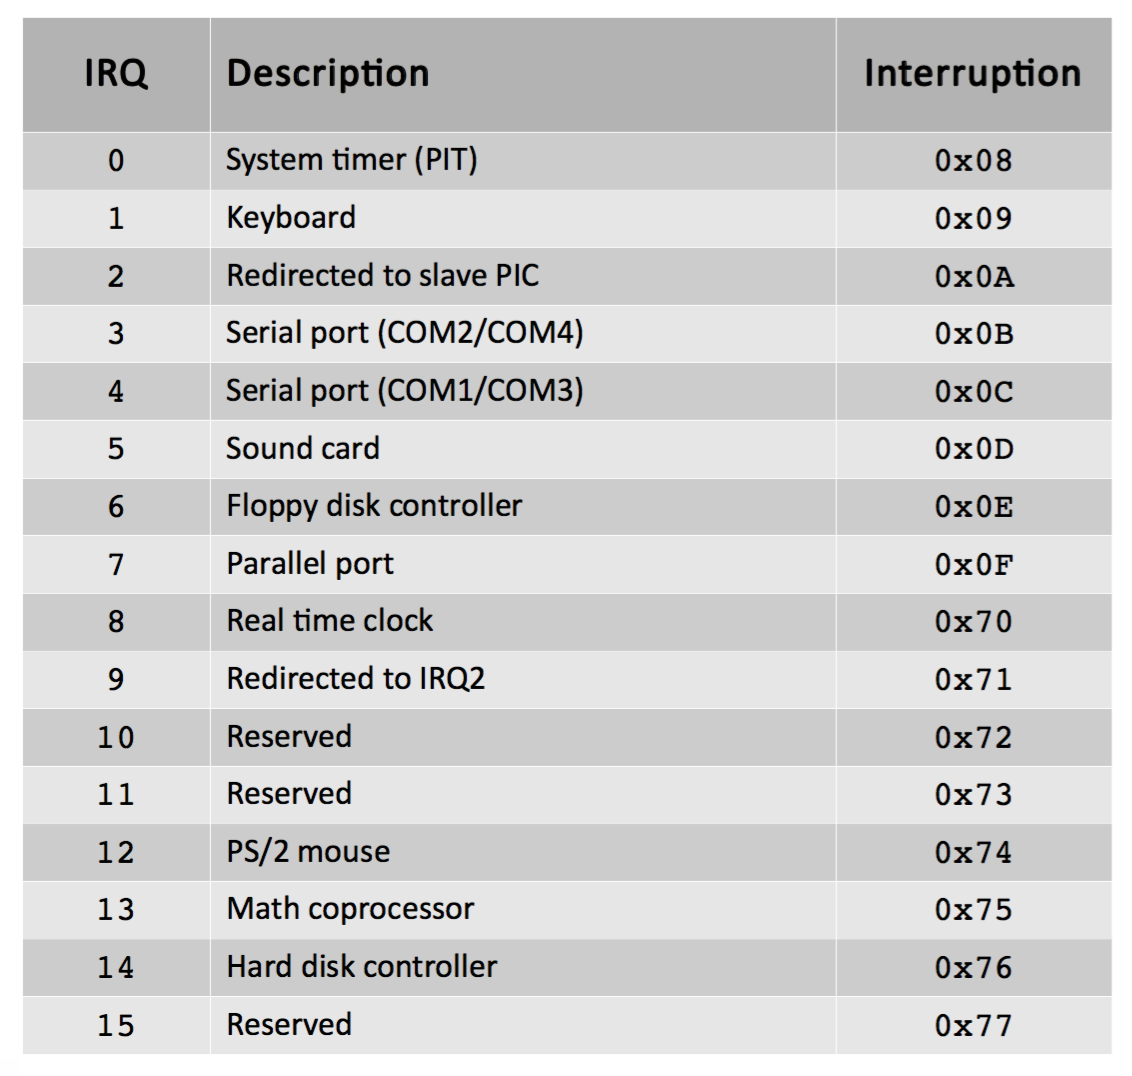
\includegraphics[scale=0.5]{images/irqs.png}
  \caption{Table de correspondance des \acrshort{irq}s}
  \label{irqs}
\end{figure}

En comparant la figure \ref{table_int_exc} avec la figure \ref{irqs}, on constate
que certaines \acrshort{irq}s partagent le même numéro d'interruption que des
exceptions. L'interruption du \textit{timer} par exemple a le même numéro d'interruption
que l'exception \textit{Double Fault} (0x8). Si on laisse le \textit{mapping} par
défaut, une interruption du \textit{timer} va déclencher une \textit{Double Fault}
ce qui n'est pas souhaitable. Il a donc été nécessaire de changer cette table
de correspondance. Les \acrshort{irq}s 0 à 7 ont été associées aux interruptions
32 à 39 et les \acrshort{irq}s 8 à 15 ont été associées aux interruptions 40 à 47.
Ce changement de \textit{mapping} peut se faire assez simplement en assembleur en
utilisant les ports des deux \acrshort{pic}s utilisés par les \acrshort{irq}s.
Un code d'exemple est donné sur le site OSDev \cite{ref22}.

%%%%%%%%%%%%%%%%%%%%%%%%%%%%%%%%%%%%%%%%%%%%%%%%%%%%%%%%%%%%%%%%%%

\subsubsection{\acrshort{idt}}
\label{idt}
La table des descripteurs d'interruption (ou \acrshort{idt}) est similaire à la
\acrshort{gdt} (la table des descripteurs globaux). Elle est aussi composée de
descripteurs de 64-bits permettant chacun de référencer une interruption. Un
descripteur est composé d'un offset indiquant l'adresse de l'\acrshort{isr} (la
routine d'interruption), un selecteur de segment indiquant le segment où se trouve
le code de l'\acrshort{isr} et un niveau de privilège indiquant le niveau de privilège
requis pour exécuter l'\acrshort{isr}. Dans le cas d'un adressage de type \textit{FLAT}
comme celui utilisé, le selecteur de segment sera forcément le selecteur de segment
de code. Il existe aussi plusieurs types de descripteurs d'interruptions \cite{ref66}
décrits dans la figure \ref{idt_entry}. Dans le cas de notre \textit{kernel} seulement
deux types ont été utilisés, le type \textit{Interrupt Gate} et le type \textit{Trap Gate}.
La différence entre un \textit{Interrupt Gate} et un \textit{Trap Gate} est uniquement
le comportement du \acrshort{cpu} lors de l'exécution de l'\acrshort{isr}\cite{ref42}.
Dans le cas du \textit{Interrupt Gate}, le \acrshort{cpu} masquera les interruptions
lors de l'exécution de l'\acrshort{isr} alors que dans un \textit{Trap Gate} ce
ne sera pas le cas. \\

\begin{figure}[!h]
  \centering
  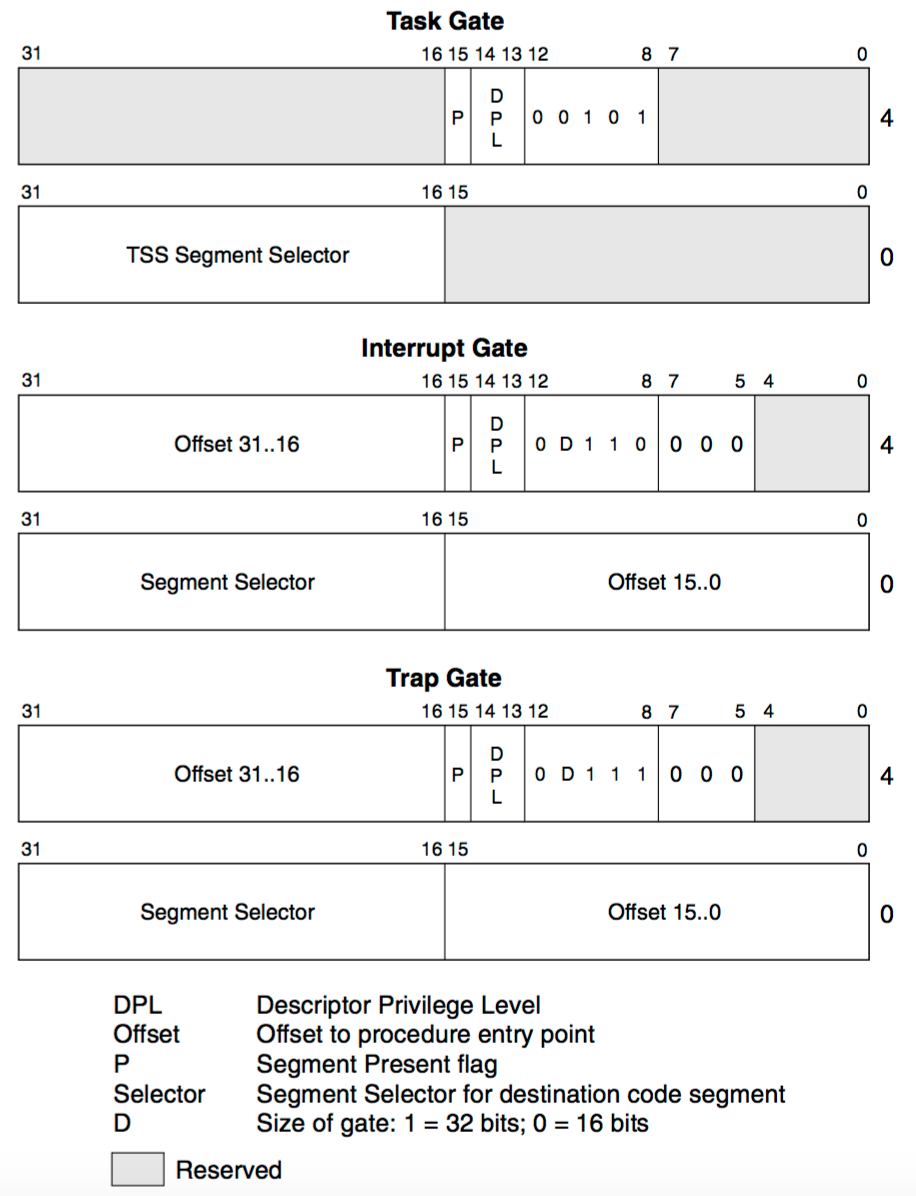
\includegraphics[scale=0.75]{images/idt_entry.png}
  \caption{Différents types de descripteur d'interruption}
  \label{idt_entry}
\end{figure}

Comme pour la \acrshort{gdt}, l'\acrshort{idt} est stockée en \acrshort{ram}
et doit donc être initialisée et gérée par l'\acrshort{os}. De la même manière
que l'instruction \mintinline{text}{LGDT} permet de charger la \acrshort{gdt},
l'instruction \mintinline{text}{LIDT} permet de charger l'\acrshort{idt} dans le
registre IDTR. Pour se faire il faut donner comme argument à l'instruction 
\mintinline{text}{LIDT} l'adresse du descripteur d'\acrshort{idt} sur 48 bits.
Ce descripteur est composé de l'adresse de l'\acrshort{idt} sur 32 bits et de sa
limite (sa taille en bytes - 1) sur 16 bits. Une fois la table des descripteurs
d'interruption chargée avec l'instruction \mintinline{text}{LIDT}, les interruptions
peuvent être activées en utilisant l'instruction \mintinline{text}{STI}. La figure
\ref{idtr} permet de résumer la relation entre le registre IDTR et l'\acrshort{idt}.

\begin{figure}[!h]
  \centering
  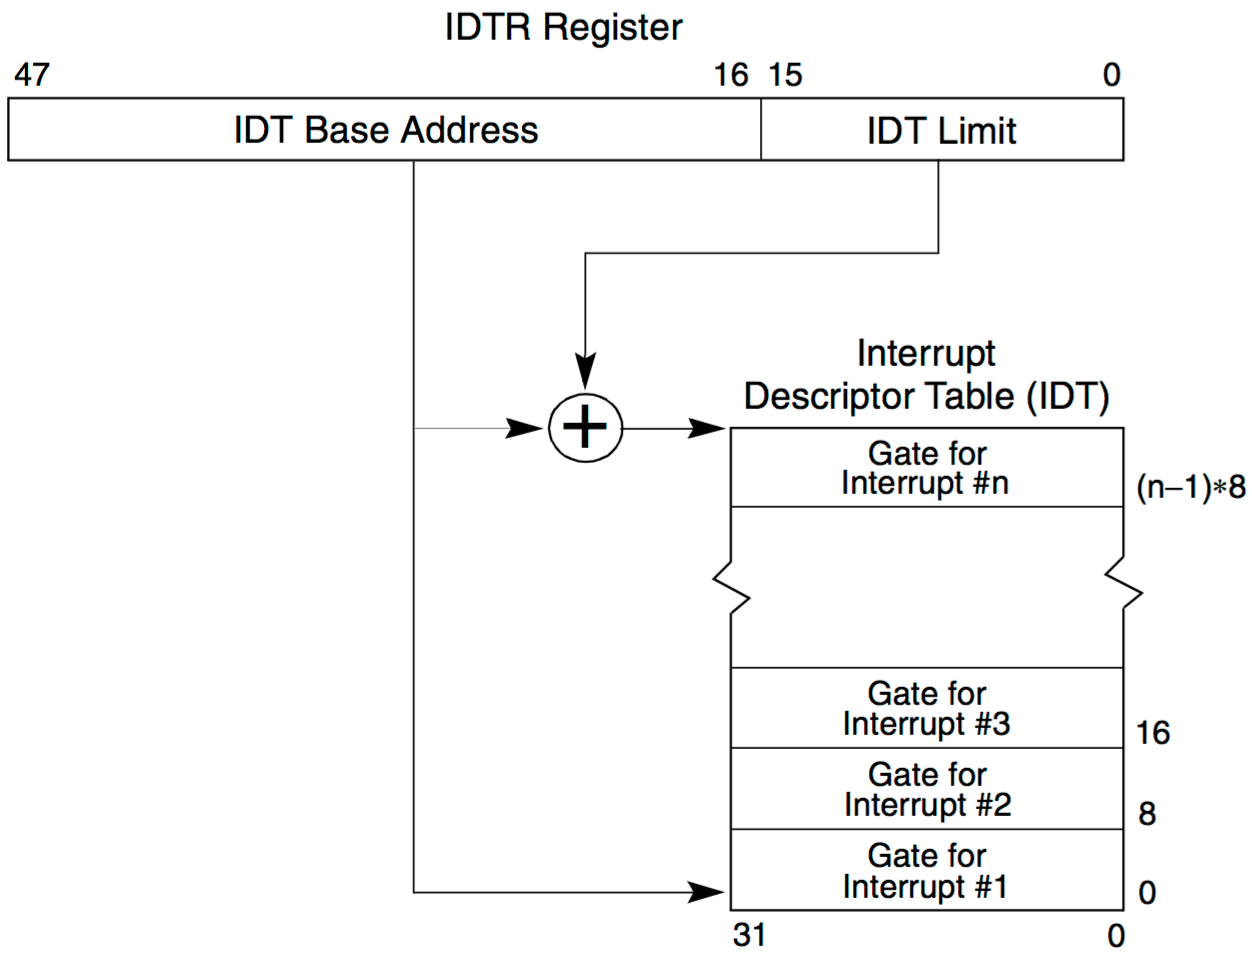
\includegraphics[scale=0.6]{images/idtr.png}
  \caption{Relation entre le registre IDTR et l'\acrshort{idt}}
  \label{idtr}
\end{figure}

Dans le \textit{kernel} développé, l'\acrshort{idt} est une structure statique
en mémoire. Une fonction assembleur est donc appelée afin de charger cette
structure dans le registre IDTR. En plus du chargement de l'\acrshort{idt}, une
partie des routines d'interruptions est faite en assembleur. En effet, il a été
nécéssaire de passer par du code bas niveau car avant de rentrer dans une
routine d'interruption, il faut sauvegarder le contexte. Il est obligatoire
de sauvegarder le contexte car, comme déjà dit plus haut, une interruption
peut avoir lieu à n'importe quel moment. La partie bas niveau de la routine
d'interruption s'occupe donc de sauvegarder le contexte puis d'appeler un
gestionnaire d'interruption haut niveau en rust. Ce gestionnaire prend comme argument
le numéro d'interruption et appelle la routine d'interruption liée à cette interruption.
Par exemple, la routine d'interruption du \textit{timer} va simplement incrémenter
un compteur. Lorsque une exception est levée le même mécanisme est employé sauf
qu'ici le \textit{kernel} va afficher un message d'erreur en fonction du numéro
de l'exception.

%%%%%%%%%%%%%%%%%%%%%%%%%%%%%%%%%%%%%%%%%%%%%%%%%%%%%%%%%%%%%%%%%%
%%%%%%%%%%%%%%%%%%%%%%%%%%%%%%%%%%%%%%%%%%%%%%%%%%%%%%%%%%%%%%%%%%

\subsection{\acrshort{vga}}
Un \acrshort{pc} possède généralement une carte graphique permettant de gérer
l'affichage. Une grande majorité des carte graphiques, même modernes sont compatibles
avec le standard d'affichage \acrshort{vga}. Dans notre cas, nous utilisons un
émulateur (QEMU) qui va émuler l'affichage \acrshort{vga}. Pour écrire sur l'écran
il faut écrire dans la mémoire vidéo (\acrshort{vram}) qui commence à l'adresse
0xA0000 et finit à l'adresse 0xBFFFF. Différents modes d'écriture existent pour
l'affichage mais nous allons nous concentrer sur un seul en particulier. \\

Le mode texte \acrshort{vga} a été utilisé pour l'affichage dans l'\acrshort{os}
développé. En mode texte, l'écran est divisé en caractères plutôt qu'en pixels ce
qui permet d'afficher simplement et rapidement quelque chose sur l'écran. La mémoire
vidéo reservée au mode texte commence à l'adresse 0xB8000 et a une taille de
$80 \times 25$ caractères. Un caractère est représenté par 2 octets (16 bits) ce
qui fait une taille de 4000 octets ($80 \times 25 \times 2$). L'octet de poids
faible d'un caractère représente la valeur ASCII de ce caractère et l'octet de poids
fort représente l'attribut qui contient lui même la couleur du caractère et la
couleur du fond (voir figure \ref{vga_char}) \cite{ref42}. La couleur en mode texte
est donc codée sur 4 bits ce qui fait 16 couleurs différentes. Ces 16 couleurs sont
décrites dans la figure \ref{colors} \cite{ref19}. \\

\begin{figure}[!h]
  \centering
  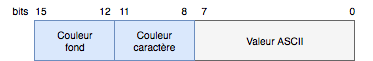
\includegraphics[scale=0.8]{images/vga_char.png}
  \caption{Structure d'un caractère en mode texte \acrshort{vga}}
  \label{vga_char}
\end{figure}

\begin{figure}[!h]
  \centering
  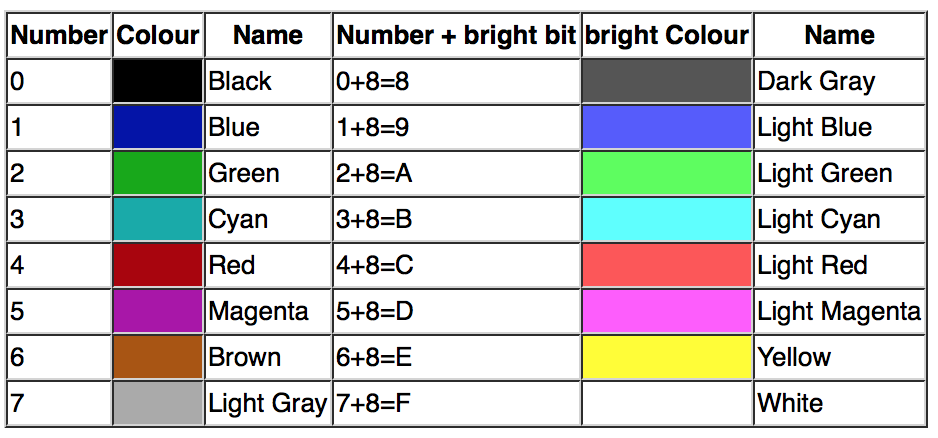
\includegraphics[scale=0.65]{images/colors.png}
  \caption{Couleurs disponibles en mode texte \acrshort{vga}}
  \label{colors}
\end{figure}

Le mode texte \acrshort{vga} permet aussi d'afficher un curseur. Le curseur ne
se déplace pas automatiquement quand un caractère est écrit à l'écran, c'est
simplement une zone de l'écran mise en évidence par un clignotement et dont
la taille, la position et la visibilité peuvent être modifiés \cite{ref23}. L'accès
au curseur se fait en utilisant les registres du \acrshort{crtc} (\textit{Cathode Ray
Tube Controller}). Les registres du \acrshort{crtc} peuvent être accédés avec la
paire registre d'adresse et registre de données. Ces regsitres se trouvent respectivement
aux ports 0x3D4 et 0x3D5. L'écriture dans un registre du \acrshort{crtc} se fait
donc en deux temps. Tout d'abord, l'adresse du registre doit être specifiée
en écrivant dans le port 0x3D4 puis la donnée doit être écrite dans le port 0x3D5
\cite{ref42}. \\

Pour l'implémentation du support \acrshort{vga} dans le \textit{kernel} plusieurs
structure ont été créées. Tout d'abord, la couleur est représentée par un simple
\mintinline{rust}{enum}. Une structure pour l'attribut a ensuite été écrite
dont le constructeur prend comme argument la couleur de fond et la couleur du
caractère. Après cela, une structure représentant un caractère sur 16 bits a été
implémentée. Cette structure est composée du caractère sur 8 bits et de l'attribut
sur 8 bits aussi. Ces structures permettent de simplifier la construction d'un
caractère pour l'écrire dans le \textit{frame buffer} (mémoire vidéo dédiée au
mode texte \acrshort{vga}). Une dernière structure a finalement été créée
comportant un \textit{raw pointer} vers le \textit{frame buffer} (qui est un
tableau de $80 \times 25$ caractères) ainsi que les informations sur la couleur
et la position du curseur. Si la pagination est active comme c'est le cas dans
notre \acrshort{os}, il faut bien penser à mettre l'adresse virtuelle du
\textit{frame buffer} (0xB8000 étant l'adresse physique).

\begin{code}
\begin{minted}[fontsize=\footnotesize,tabsize=4,frame=single,linenos]{rust}
static mut SCREEN: Screen = Screen {
    buffer: 0xC00B8000 as *mut _,
    attribute: ColorAttribute::new(Color::White, Color::Black),
    cursor_x: 0,
    cursor_y: 0
};
\end{minted}
\caption{Structure \mintinline{rust}{Screen}}
\label{lst:vga:struct}
\end{code} \bigbreak

La structure \mintinline{rust}{Screen} est déclarée statiquement dans le \textit{kernel}
ce qui rend tout appel à une méthode \mintinline{rust}{unsafe} pour rust. En plus
des méthodes pour manipuler cette structure, des fonctions ont donc été implémentées
afin d'interfacer l'écriture sur l'écran. Ces fonctions permettent en plus d'éviter
de mettre le code en \mintinline{rust}{unsafe} à chaque fois que l'on veut afficher
quelque chose. En rust, les macros \mintinline{rust}{print} et \mintinline{rust}{println}
écrivent sur la sortie standard. Etant donné que nous sommes dans une configuration
\textit{bare-metal}, nous n'avons pas de sortie standard et ces deux macros n'existent
pas. Si nous étions en C, l'équivalent de ces macros aurait été la fonction
\mintinline{c}{printf} et nous aurions eu à la coder entièrement. Heureusement,
rust facilite grandement les choses avec le \mintinline{rust}{trait Write}.
Pour implémenter ce \mintinline{rust}{trait} dans une structure, il faut simplement
lui indiquer comment écrire une chaîne de caractères ce qui a donc été fait
pour la structure \mintinline{rust}{Screen}. L'implémentation de ce \mintinline{rust}{trait}
par une structure donne accès à cette dernière à de nombreuses méthodes mais celle
qui nous intéresse ici est la méthode \mintinline{rust}{write_fmt}. Cette méthode
prend en paramètre une structure \mintinline{rust}{Arguments}. La structure
\mintinline{rust}{Arguments} permet la gestion des arguments en ligne de commande
ou les macros à arguments variable. La macro \mintinline{rust}{print} possède
un nombre d'arguments variable, nous pouvons donc implémenter cette macro ainsi
que la macro \mintinline{rust}{println} comme suit :

\begin{code}
\begin{minted}[fontsize=\footnotesize,tabsize=4,frame=single,linenos]{rust}
macro_rules! print {
    ($($arg:tt)*) => (vga_write_fmt(format_args!($($arg)*)));
}

macro_rules! println {
    () => (print!("\n"));
    ($fmt:expr) => (print!(concat!($fmt, "\n")));
    ($fmt:expr, $($arg:tt)*) => (print!(concat!($fmt, "\n"), $($arg)*));
}
\end{minted}
\caption{Implémentation des macros \mintinline{rust}{print} et \mintinline{rust}{println}}
\label{lst:vga:print}
\end{code} \bigbreak

A noter que la fonction \mintinline{rust}{vga_write_fmt} est simplement une fonction
interfaçant la méthode \mintinline{rust}{write_fmt} appliquée à la structure
\mintinline{rust}{Screen} et la macro \mintinline{rust}{format_args} convertie
les arguments de la macro \mintinline{rust}{print} en structure \mintinline{rust}{Arguments}.

%%%%%%%%%%%%%%%%%%%%%%%%%%%%%%%%%%%%%%%%%%%%%%%%%%%%%%%%%%%%%%%%%%
%%%%%%%%%%%%%%%%%%%%%%%%%%%%%%%%%%%%%%%%%%%%%%%%%%%%%%%%%%%%%%%%%%

\subsection{\textit{Timer}}
Dans chaque \acrshort{pc} se trouve une puce pour mesure le temps et implémenter
des \textit{timers} \cite{ref42}. Cette puce est le \textit{Programmable Interval Timer}
(\acrshort{pit}). Sur architecture \acrshort{IA-32}, le \acrshort{pit} est générallement
un Intel 8253 et dans notre cas, c'est celui émulé par QEMU. Le \acrshort{pit}
génère une interruption matérielle (\acrshort{irq}0) à une fréquence sélectionnable
entre 18.2065 Hz et 1.19318 MHz. L'horloge du \acrshort{pit} oscille à 1.19318 MHz.
La fréquence de sortie est modulée à l'aide d'un diviseur configurable par le
\textit{kernel}. Ce diviseur est une valeur sur 16 bits. Sa valeur maximale est
donc 65536 ce qui explique la valeur minimale de la fréquence du \acrshort{pit}
($\frac{1193180}{65536} \simeq 18.2065$). Le \acrshort{pit} possède aussi plusieurs
canaux avec chacun un diviseur propre mais seulement le premier canal (canal 0)
est utilisé dans le \textit{kernel} est c'est sur celui-ci que nous allons nous
concentrer. Le \acrshort{pit} est programmable à l'aide de différents ports.
Le port 0x43 contient le registre de commande du \acrshort{pit} et le port 0x40
permet de configurer le canal 0. Ci-dessous, le code permettant de programmer
le \textit{timer} à une fréquence \mintinline{rust}{freq}.

\begin{code}
\begin{minted}[fontsize=\footnotesize,tabsize=4,frame=single,linenos]{rust}
let div = 1193180 / freq;
outb(0x43, 0x36);
outb(0x40, (div & 0xFF) as u8);
outb(0x40, (div >> 0x8) as u8);
\end{minted}
\caption{Programmation du \textit{timer} en assembleur}
\label{lst:timer:init}
\end{code} \bigbreak

Ecrire 0x36 dans le registre de commande du \acrshort{pit} indique la sélection
du diviseur et le mode répétition  (réinitialisation du compteur une fois celui-ci
arrivé à 0) \cite{ref42}. L'octet de poids faible du diviseur est ensuite écrit
dans le port du canal 0 suivi par l'octet de poids fort. Dans le \textit{kernel}
développé, le \textit{timer} est représenté par une structure statique contenant
la fréquence du timer sur 32 bits et l'état actuel de son compteur sur 32 bits.
Ce compteur est incrémenté à chaque fois qu'une interruption à lieu sur l'\acrshort{irq}0.
Comme pour la structure statique permettant d'interfacer l'affichage texte \acrshort{vga},
toute modification de celle du \textit{timer} sera \mintinline{rust}{unsafe}
au niveau du compilateur rust. Des fonctions ont donc été implémentées pour lire
ou écrire le \textit{timer}. Actuellement, le \acrshort{pit} est utilisé seulement
pour arrêter le \textit{kernel} pendant un temps donné avec la fonction \mintinline{rust}{sleep}.
Cette fonction prend une durée en millisecondes et rentre dans une boucle (attente
active).

\begin{code}
\begin{minted}[fontsize=\footnotesize,tabsize=4,frame=single,linenos]{rust}
pub fn sleep(ms: u32) {
    let duration = get_ticks() + (ms * get_freq() / 1000);
    loop {
        if get_ticks() >= duration {
            break;
        }
        halt();
    }
}
\end{minted}
\caption{Implémentation de la fonction \mintinline{rust}{sleep}}
\label{lst:timer:sleep}
\end{code} \bigbreak

Ici, \mintinline{rust}{get_ticks} et \mintinline{rust}{get_freq} sont des fonctions
qui renvoient les attributs \mintinline{rust}{ticks} et \mintinline{rust}{freq}
de la structure statique précédemment décrite. La fonction \mintinline{rust}{halt}
appelle l'instruction assembleur \mintinline{text}{HLT} qui arrête le processeur
jusqu'à ce qu'une interruption matérielle soit déclenchée. Elle est appelée après
chaque comparaison pour éviter d'utiliser $100\%$ du \acrshort{cpu} lors de l'attente
sur un \mintinline{rust}{sleep}. On pourrait imaginer d'autres utilisations du
\textit{timer} comme par exemple la génération de nombres pseudo-aléatoires.

%%%%%%%%%%%%%%%%%%%%%%%%%%%%%%%%%%%%%%%%%%%%%%%%%%%%%%%%%%%%%%%%%%
%%%%%%%%%%%%%%%%%%%%%%%%%%%%%%%%%%%%%%%%%%%%%%%%%%%%%%%%%%%%%%%%%%

\subsection{Clavier}
Afin d'avoir un système d'exploitation un minimum complet, il est impératif
de faire un support pour le clavier. Sur architectur Intel 32-bits, chaque
pression ou relâchement d'une touche du clavier déclenche une interruption
matérielle (\acrshort{irq}1) \cite{ref42}. Le périphérique clavier possède un
\textit{buffer} interne qui va stocker les données à chaque interruption. Ces données
sont appelées \textit{scan codes}. Chaque \textit{scan code} correspond à une
touche du clavier et le bit de poids fort du \textit{scan code} indique si
la touche a été pressée (\textit{make code}) ou relâchée (\textit{break code}).
La valeur de la touche est stockée dans les sept bits de poids faible mais n'est
pas à confondre avec un code ASCII (figure \ref{scancode}). Il faut donc faire
correspondre la valeur chaque touche avec une valeur ASCII ce qui a été fait avec
une table de correspondance dans le \textit{kernel}.

\begin{figure}[!h]
  \centering
  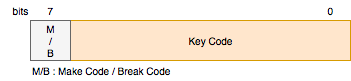
\includegraphics[scale=0.8]{images/scancode.png}
  \caption{Structure d'un \textit{scan code}}
  \label{scancode}
\end{figure}

Le clavier comporte deux registres. Un registre de données et un registre d'état.
Ces registres sont accessibles par les ports 0x60 et 0x64. Lors d'une interruption,
le \textit{scan code} de la touche est stockée dans le registre de données. Avant
de lire une donnée venant du clavier, il est nécessaire de s'assurer que le
\textit{buffer} du clavier ne soit pas vide en en venant lire le registre d'état.
Normalement si une interruption a eu lieu, cela veut dire que le \textit{buffer}
est plein mais il est quand même important de vérifier pour éviter toute source
d'erreur. Une donnée est prête à être lue si le bit 0 (bit de poids faible) du
registre d'état est à 1. Ci-dessous, un exemple de routine d'interruption stockant
la valeur ascii du \textit{scan code} dans un \textit{buffer}.\\

\begin{code}
\begin{minted}[fontsize=\footnotesize,tabsize=4,frame=single,linenos]{rust}
pub fn keyboard_handler() {
    let state = inb(0x64) & 1;
    if state == 1 {
        let key = inb(0x60);
        if key >> 7 == 0 {
            buffer_write(KEY_MAP[key as usize])
        }
    }
}
\end{minted}
\caption{Routine d'interruption du clavier}
\label{lst:keyboard:handler}
\end{code} \bigbreak

Au niveau de l'implémentation logicielle, un \textit{buffer} circulaire a été
utilisé pour la gestion du clavier. Un \textit{buffer} circulaire est un \textit{buffer}
de taille fixe dont la fin est connectée au début. Ce type de structure de donnée
est bien adapté aux flux constants de données comme la gestion d'un clavier.
A chaque fois qu'une touche va être lue par la routine d'interruption du clavier,
cette dernière va être stockée dans le \textit{buffer}. La case du \textit{buffer}
contenant cette donnée est considérée comme libre si elle a été lue. Le \textit{buffer}
circulaire va donc permettre de gérer un nombre d'écritures supérieur au nombre
de lectures.